\subsection{RQ3: Test Code Maintenance}

We next address RQ3 of whether test generalization can reduce the efforts in maintaining test code. We use two metrics to address this research question. First, we compare the number of CUTs and the number of PUTs. The higher the difference between the number of CUTs and the number of PUTs, the lesser are the efforts required in maintaining the test code.
The reason is that whenever the code under test is modified, all failing tests need to be modified based on the new expected behavior of the code under test. Therefore, lower number of PUTs can significantly reduce the efforts in maintaining the test code since only a few PUTs need to be modified. Second, we compare the Lines of Code (LOC) of CUTs and PUTs. The reason for the second metric is that lower number of PUTs with a high amount of LOC does not help in reducing the efforts required in maintaining the test code.

\begin{figure}[t]
\centering
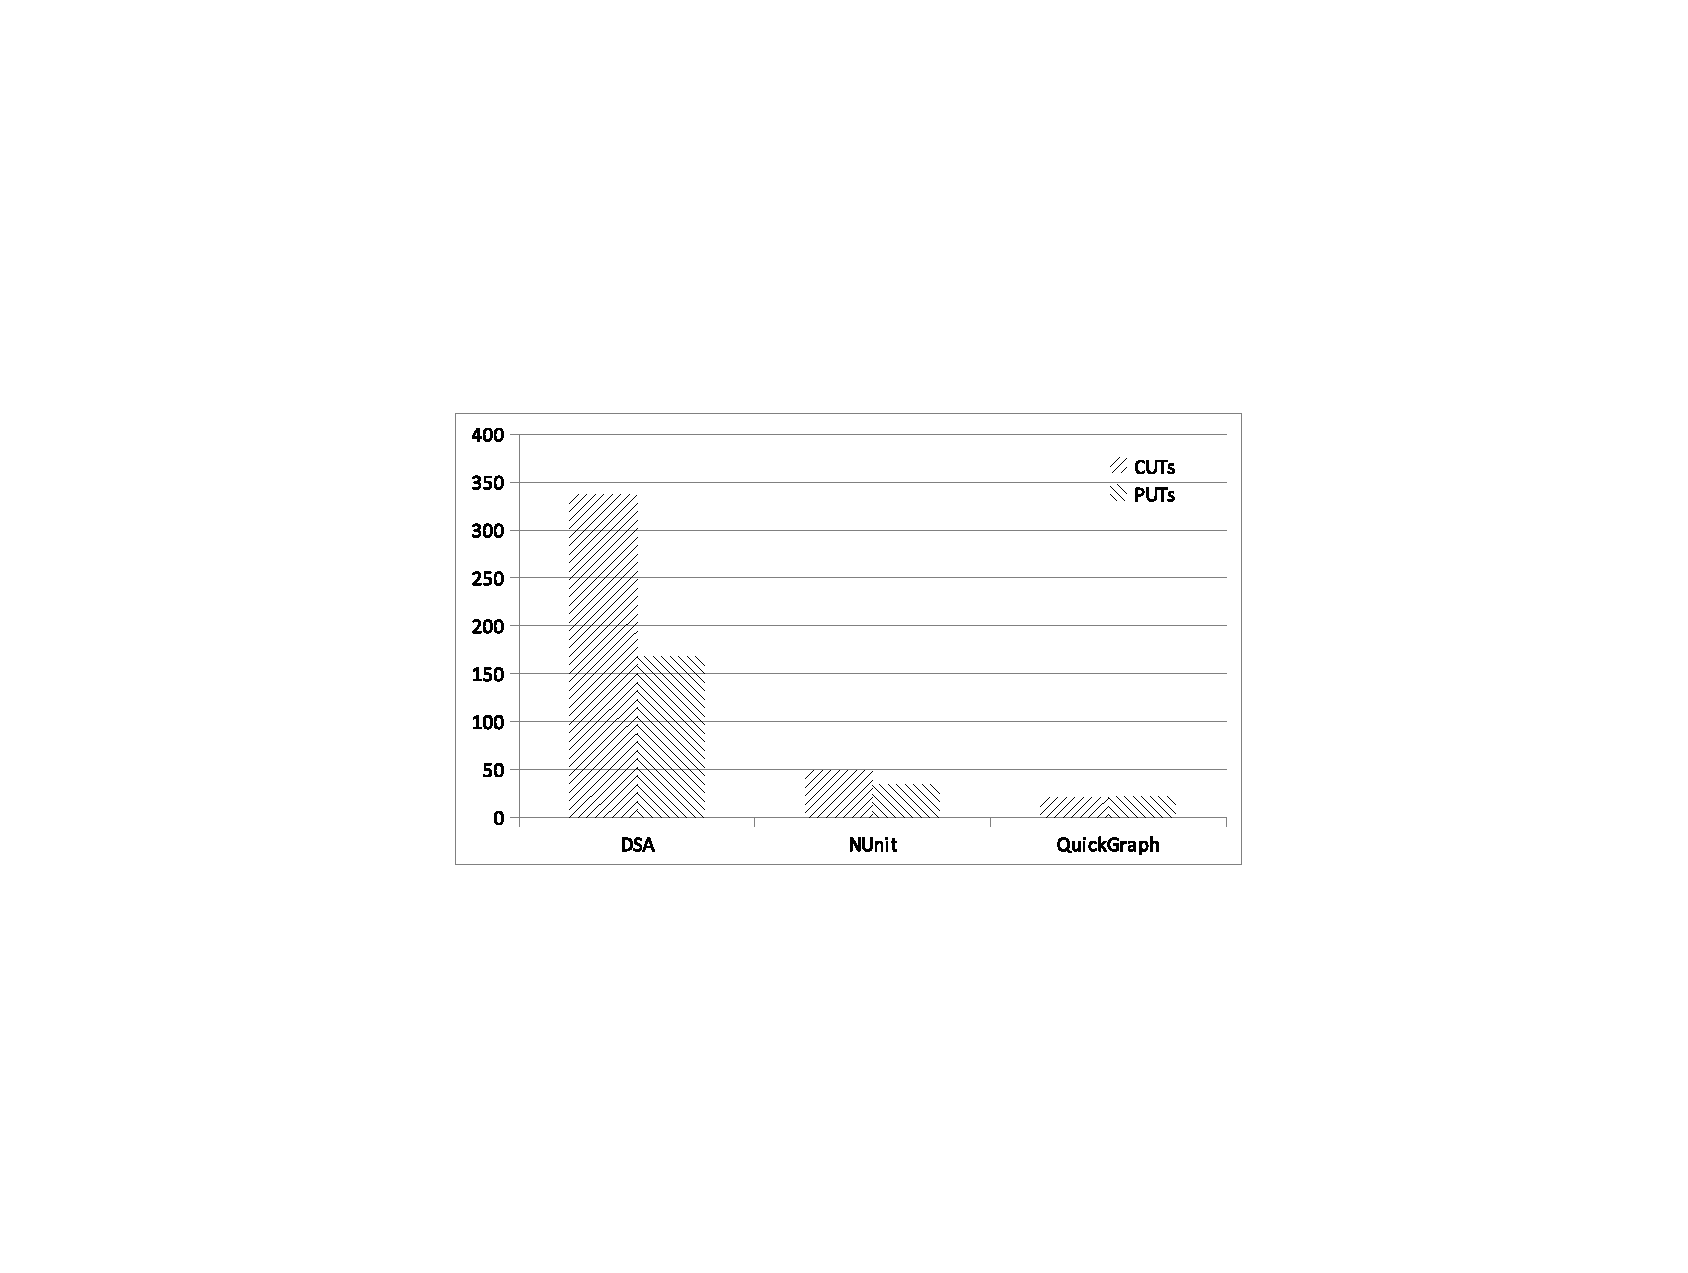
\includegraphics[scale=0.45,clip]{charts/CUTs_PUTs_1.eps}\vspace*{-1ex}
\caption{\label{fig:cutsnputs}Comparison of the number of CUTs and PUTs} \vspace*{-1ex}
\end{figure}

\begin{table}[t]
\begin{CodeOut}
\begin{center}
\centering 
\begin {tabular} {|c|c|c|}
\hline \textbf{CUT} & \textbf{PUT} & \textbf{\# of occurrences}\\
\hline
\hline 1   & 1   & 129\\
\hline 1   & 2   & 2\\
\hline 1   & 3   & 2\\
\hline 2   & 1   & 29\\
\hline 3   & 1   & 14\\
\hline 4   & 1   & 15\\
\hline 5   & 1   & 4\\
\hline 6   & 1   & 4\\
\hline 7   & 1   & 1\\
\hline 8   & 1   & 2\\
\hline 9   & 1   & 1\\
\hline 15   & 1   & 1\\
\hline
\end{tabular}\vspace*{-2ex}
\caption {\label{tab:cutputmapping} Mapping of the number of CUTs and their transformed PUTs.} \vspace*{-5ex}
\end{center}
\end{CodeOut}
\end{table}

Figure~\ref{fig:cutsnputs} shows the comparison of the number of CUTs with PUTs for all subject applications. The x-axis shows the subject application and y-axis shows the number of CUTs or PUTs. In total, we generalized $407$ CUTs to $224$ PUTs that achieved a higher code coverage than CUTs and also detected new defects that are not detected by the CUTs. The figure shows that there is a significant reduction in the number of tests for the subjects DSA and NUnit. This reduction in the number of tests is because multiple CUTs are generalized to a single PUT. Table~\ref{tab:cutputmapping} shows the mappings between the number of CUTs and their transformed PUTs. For example, Row 1 shows that one CUT is transformed to one PUT in 129 occurrences. Similarly, the last row shows that 15 CUTs are transformed into a single PUT in one occurrence. Rows 2 and 3 show exceptional cases where a CUT is generalized to more than one PUT. Section~\ref{sec:limitations} discusses more about these exceptional cases. 

Figure~\ref{fig:transformedPUT} shows an example PUT, which is a result of generalizing four CUTs of the \CodeIn{SinglyLinkedList} class of DSA. The objective of all four CUTs is to test the \CodeIn{AddFirst} method (method under test) that adds an element to a list object of type \CodeIn{SinglyLinkedList}. These four CUTs verify different behaviors by adding one element or two elements to a list and by verifying whether the \CodeIn{head} and \CodeIn{tail} values of the list are updated correctly. We generalized all these four CUTs into a single PUT shown in Figure~\ref{fig:transformedPUT}. The CUTs verify the behavior of the \CodeIn{AddTest} method by adding only a fixed number of elements (with fixed values) to the list. In contrast, our PUT can verify the behavior of the \CodeIn{AddFirst} method with variable number of elements in the list. 

\begin{figure}[t]
\begin{CodeOut}
\begin{alltt}
public void AddFirstTest([PAUT]SinglyLinkedList<int> sll, 
\hspace*{0.6in}[PAUT]int[] ne) \{            
\hspace*{0.2in}PexAssume.IsTrue(ne.Length > 1);
\hspace*{0.2in}PexAssume.IsTrue(sll.Count == 0);
\hspace*{0.2in}for (int i = 0; i < ne.Length; i++)
\hspace*{0.4in}sll.AddFirst(ne[i]);
\hspace*{0.2in}PexAssert.AreEqual(ne[ne.Length - 1], sll.Head.Value);            
\hspace*{0.2in}PexAssert.AreEqual(ne[0], sll.Tail.Value);
\hspace*{0.2in}PexAssert.AreEqual(ne.Length, sll.Count);
\}
\end{alltt}
\end{CodeOut}\vspace*{-4ex}
\Caption{\label{fig:transformedPUT} The \CodeIn{AddFirstTest} PUT for the \CodeIn{AddFirst} method under test.}
\end{figure}

Figure~\ref{fig:loccomp} shows the results of comparing LOC of CUTs and PUTs. For DSA, LOC of PUTs is less than the LOC of CUTs, whereas for the other two subjects, LOC of PUTs is slightly more than the LOC of CUTs. We identify that among new LOC written for PUTs, many statements are related to the additional \CodeIn{using} statements or new annotations added during our test generalization. On an average, LOC of PUTs is almost the same as the LOC of CUTs. Therefore, our results show that test generalization can help reduce the number of tests and thereby reduce the efforts in maintaining test code.

\begin{figure}[t]
\centering
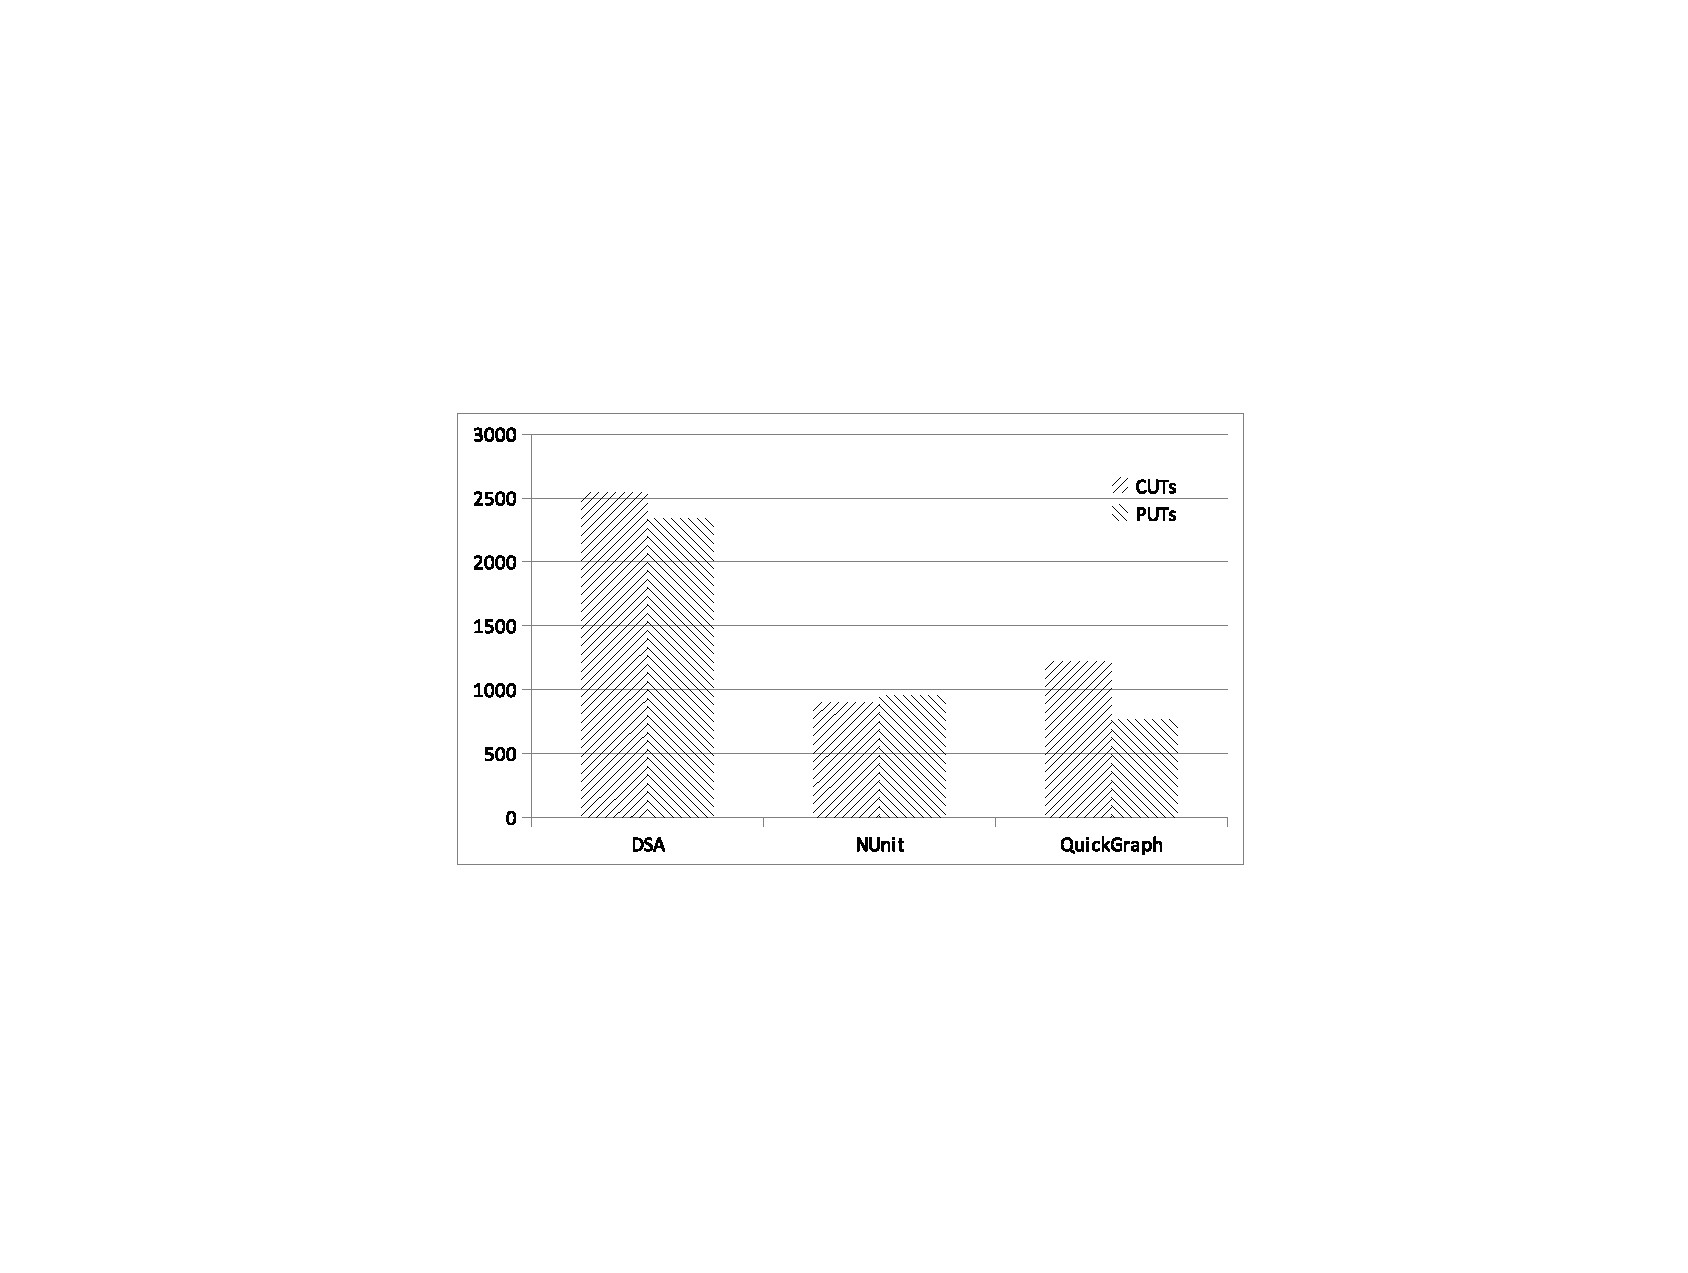
\includegraphics[scale=0.45,clip]{charts/LOC_1.eps}\vspace*{-1ex}
\caption{\label{fig:loccomp}Comparison of Lines of Code of CUTs and PUTs} \vspace*{-2ex}
\end{figure}
